
\section{Experimental Setup}
\label{sec:exp-setup}

We evaluate our method on 4 multi-step QA datasets in the open-domain setting: \textbf{HotpotQA}~\cite{hotpotqa}, \textbf{2WikiMultihopQA}~\cite{xanh2020_2wikimultihop}, answerable subset of \textbf{MuSiQue}~\cite{musique}, and answerable subset of \textbf{IIRC}~\cite{iirc}. For HotpotQA, we use the Wikipedia corpus that comes with it for the open-domain setting. For each of the other three datasets, which originally come in a reading comprehension or mixed setting, we used the associated contexts to construct a corpus for our open-domain setting (see App.~\ref{sec:apndx-corpora} for details). For each dataset, we use 100 randomly sampled questions from the original development set for tuning hyperparameters, and 500 other randomly sampled questions as our test set.


\subsection{Models}
\label{subsec:exp-models}

\paragraph{Retriever.} We use BM25~\cite{bm25} implemented in Elasticsearch\footnote{\url{https://www.elastic.co/}} as our base retriever. We compare two retriever systems:

(i) \textbf{One-step Retriever (OneR)} uses the question as a query to retrieve $K$ paragraphs. We select $K \in \{5, 7, 9, 11, 13, 15\}$ that's best on the dev set.

(ii) \textbf{\iconsys Retriever} is our method described in \S\ref{sec:method}. We use BM25 as its underlying retriever and experiment with OpenAI GPT3 (\texttt{code-davinci-002})~\cite{originalgpt3,instructgpt3,codex} and Flan-T5~\cite{flan} of different sizes as its CoT generator.

For demonstrating in-context examples to these LMs, we wrote CoTs for 20 questions for all the datasets (see App. \S\ref{sec:apndx-prompts}). We then create 3 demonstration (``training'') sets by sampling 15 questions each for each dataset. For each experiment, we search for the best hyperparameters for the dev set using the first demonstration set and evaluate each demonstration set on the test set using the selected hyperparameters. We report the mean and standard deviation of these 3 results for each experiment.

 At test time, we pack as many demonstrations as possible within the model's context length limit. The context limit for GPT3 (\texttt{code-davinci-002}) is 8K word pieces. Flan-T5-* doesn't have any hard limit as it uses relative position embeddings. But we limit Flan-T5's context to 6K word pieces, which is the maximum we could fit in the memory of our 80G A100 GPUs.

\iconsys Retriever has one key hyperparameter: $K \in \{2, 4, 6, 8\}$, the number of paragraphs to retrieve at each step. Additionally, when creating ``training'' demonstrations for \iconsys's Reasoner module, we use gold paragraphs and a smaller number $M \in \{1, 2, 3\}$ of distractor paragraphs (\S\ref{subsec:retriever}).

\textbf{Retrieval Metric:} We allow a maximum of 15 paragraphs for all retriever systems and measure the recall of the gold paragraphs among the retrieved set of paragraphs. We search for the hyperparameter $K$ (and $M$ for \iconsys) that maximizes the recall on the dev set and use it on the test set. The reported metric can thus be viewed as the \emph{fixed-budget optimal recall} for each system considered.\footnote{\label{footnote:retrieval-metric}Note that our retrieved documents are not ranked, making standard information retrieval metrics such as MAP and DCG inapplicable. Further, we can only limit the number of retrieved paragraphs \emph{per step} to $K$. Since the total number of reasoning steps varies for questions, and in some cases, we don't even obtain all $K$ paragraphs in a given step, the total number of retrieved paragraphs also varies (even though capped at 15). This makes Recall@k, Precision@k, etc., also not applicable as metrics for any given k.}

\paragraph{QA Reader.} To implement the reader, we use the same LMs as used in the \texttt{reason-step} of \iconsys Retriever. We found that QA readers implemented with Flan-T5-* perform better with the Direct Prompting strategy and GPT3 performs better with CoT Prompting strategy (see App. ~\ref{sec:apndx-readers-results}). Hence we use Direct prompting strategy for QA with Flan-T5-* and CoT with GPT3 for the experiments.\footnote{\iconsys, by construction, produces a CoT as a part of its retrieval process. Thus, instead of having a separate post-hoc reader, one can also just extract the answer from the CoT generated during retrieval. However, we found this to be a suboptimal choice, so we always use a separate reader (see App.~\ref{sec:qa-reader-ablation}).}

The QA reader has one hyperparameter $M$: the number of distractor paragraphs in the in-context demonstrations. We search for $M$ in $\{1, 2, 3\}$. When used in conjunction with \iconsys retriever $M$ is tied for the CoT generator and the reader.

\paragraph{Open-Domain QA (ODQA) Models.} Putting retrievers and readers together, we experiment with ODQA models constructed from the various language models denoted as \textbf{OneR QA} and \textbf{\iconsys QA}. For \iconsys QA, the choice of LM for the CoT generator and the reader is kept the same. We also experiment with retriever-less QA readers \textbf{NoR QA} to assess how well LMs can answer the question from their parametric knowledge alone. To select the best hyperparameters for the ODQA model, we search for the hyperparameters $K$ and $M$ that maximize the answer F1 on the development set.


IIRC is structured slightly differently from the other datasets, in that its questions are grounded in a main passage and other supporting paragraphs come from the Wikipedia pages of entities mentioned in this passage. We slightly modify the retrievers and readers to account for this (see App.~\ref{sec:apndx-iirc-special-handling}).


\begin{figure*}[ht]
\centering
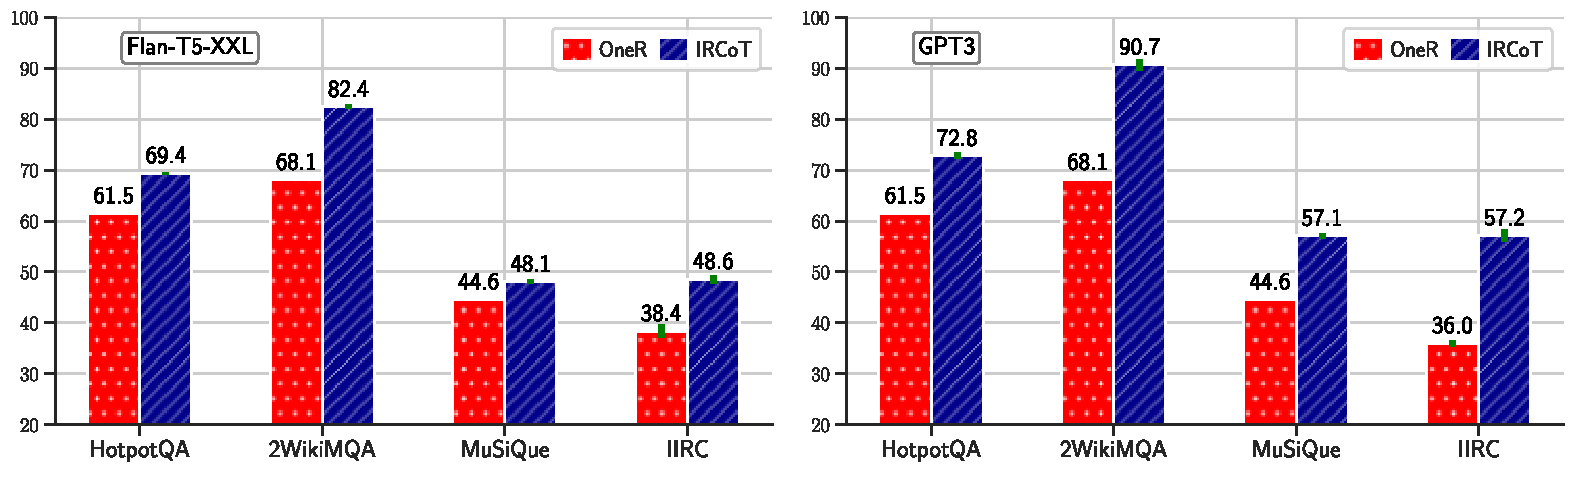
\includegraphics[width=0.95\textwidth]{images/main_retrieval_results.pdf}
\caption{Retrieval recall for one-step retriever (OneR) and \iconsys instantiated from \texttt{Flan-T5-XXL} (left) and \texttt{GPT3} (right) models. \iconsys outperforms OneR for both models and all datasets.}
\label{fig:main-retrieval-results}
\end{figure*}

\begin{figure*}[ht]
\centering
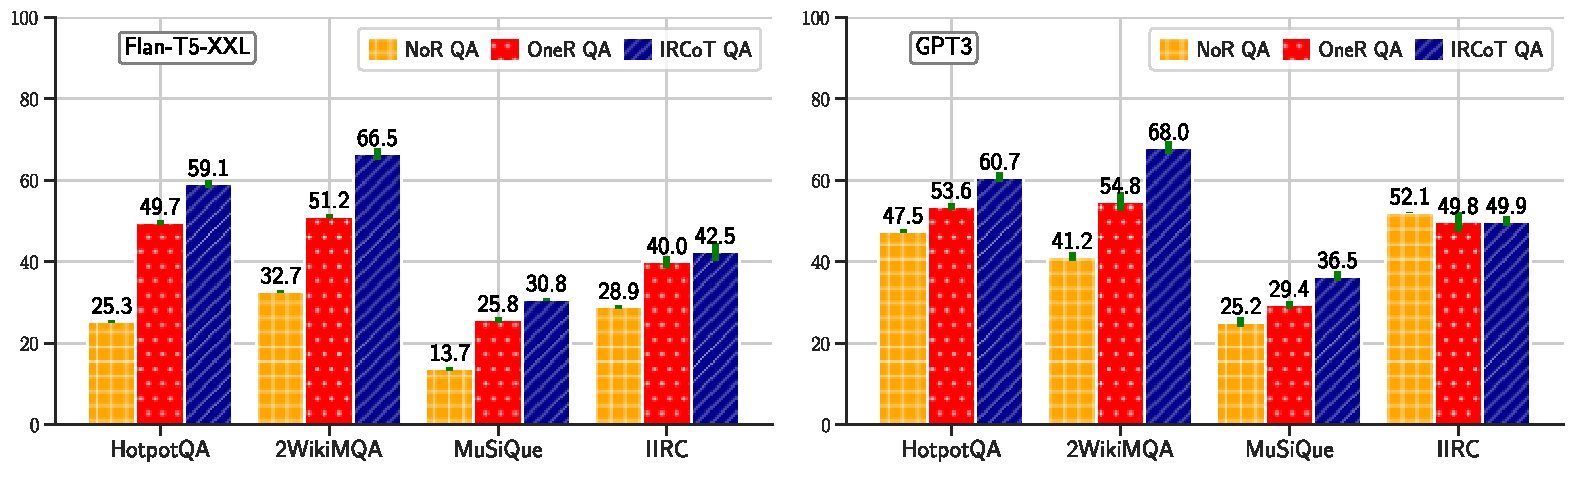
\includegraphics[width=0.95\textwidth]{images/main_qa_results.pdf}
\caption{Answer F1 for ODQA model made using (i) no retriever (NoR QA) (ii) one-step retriever (OneR QA) and (iii) \iconsys QA instantiated from \texttt{Flan-T5-XXL} (left) and \texttt{GPT3} (right) models. \iconsys QA outperforms OneR QA and NoR QA for both models on all datasets, except for GPT3 on IIRC.}
\label{fig:main-qa-results}
\end{figure*}